\documentclass[11pt]{article}
\usepackage[textwidth=15cm,textheight=22cm]{geometry}
\usepackage{amsmath,amssymb,amsthm,booktabs,graphicx,array}
\usepackage[colorlinks=true,linkcolor=blue,citecolor=blue,urlcolor=blue]{hyperref}
\setlength{\emergencystretch}{2.5em}
% Use \includeprooffalse when this supplement accompanies the FULL version (its appendix already
% contains the proofs); keep \includeprooftrue for the LEAN version.
\newif\ifincludeproof \includeprooftrue
\newtheorem{result}{Result}
\renewcommand{\thetable}{S\arabic{table}}\renewcommand{\thefigure}{S\arabic{figure}}
\title{Supplementary Material for\\ ``Integrated-Haar wavelet collocation with a provably real spectrum on arbitrary grids''}
\author{Farshid Mossaiby}
\date{}
\begin{document}
\maketitle
\noindent Part~A states the results of the main text formally and proves them. Part~B contains additional
tables and a figure, all generated by the scripts of the repository \url{https://github.com/mossaiby/iHaar}.

\ifincludeproof
\section*{Part A. Statements and proofs}
\subsection*{Notation}
The grid is $a=t_0<t_1<\dots<t_N=b$, with cells $I_k=[t_{k-1},t_k]$ of width $h_k$, midpoints $m_k$ and midpoint
spacings $d_k=(h_k+h_{k+1})/2$. The trial space $\mathcal S_h$ consists of the $C^1$ quadratic splines on the
grid, $U_k=s(m_k)$ are the nodal values, and $c_k=s''|_{I_k}$ are the cell values of the second derivative.
The second-derivative operator is $D_2=A^{-1}L$, and $\delta^2$ is the three-point second-difference matrix.

\subsection*{Statements}
\begin{result}[Three-term identity and solvability]\label{thm:identity}
For every $s\in\mathcal S_h$, with $U_k=s(m_k)$ and $c_k=s''|_{I_k}$, and for $2\le k\le N-1$,
\begin{equation}\label{eq:interior}
\frac{U_{k+1}-U_k}{d_k}-\frac{U_k-U_{k-1}}{d_{k-1}}
=\frac{h_{k-1}^2}{8d_{k-1}}c_{k-1}+\Big(h_k-\frac{h_k^2}{8d_{k-1}}-\frac{h_k^2}{8d_k}\Big)c_k+\frac{h_{k+1}^2}{8d_k}c_{k+1}.
\end{equation}
At the left end, with $g_0=s(a)$,
\begin{align}
\frac{U_2-U_1}{d_1}-\frac{2(U_1-g_0)}{h_1}&=\Big(\frac{3h_1}{4}-\frac{h_1^2}{8d_1}\Big)c_1+\frac{h_2^2}{8d_1}c_2 &&\text{(value $g_0$ prescribed)},\label{eq:dirrow}\\
\frac{U_2-U_1}{d_1}&=\Big(h_1-\frac{h_1^2}{8d_1}\Big)c_1+\frac{h_2^2}{8d_1}c_2 &&\text{(if } s'(a)=0),\label{eq:neurow}
\end{align}
and symmetrically at the right end. In matrix form, $LU+b_0g_0+b_1g_1=Ac$, where $L$ is a tridiagonal
difference matrix and $A$ a tridiagonal averaging matrix.
Moreover, on every grid, $A$ has a positive diagonal, positive off-diagonal entries, and is strictly diagonally
dominant by columns; hence it is invertible. With values prescribed at both ends, the collocation
problem $s''(m_k)=f(m_k)$ has a unique solution.
\end{result}

\begin{result}[Spectrum on every grid]\label{thm:spectrum}
Let $a=t_0<t_1<\dots<t_N=b$, with $N\ge2$, be any strictly increasing knot vector. At each end, let
either the value or the slope (zero slope) be prescribed. Then $D_2=A^{-1}L$ has $N$ real and simple
eigenvalues, and it is diagonalizable with a real eigenvector matrix $V$. If a value is prescribed at
one or both ends, all eigenvalues are negative. If the slope vanishes at both ends, exactly one
eigenvalue is zero, with the constant vector as eigenvector, and all others are negative.
\end{result}

\begin{result}[Uniform grids and fourth-order correction]\label{prop:uniform}\label{thm:fourth}
On a uniform grid ($h_k\equiv h$), $D_2$ is symmetric,
\begin{equation}\label{eq:D2}
D_2=\frac{8}{h^2}\,\delta^2\,(8I+\delta^2)^{-1},
\end{equation}
where $\delta^2$ is the usual three-point second-difference matrix, with first and last diagonal entry
$-3$ for prescribed values and $-1$ for zero slope. Its eigenvectors are the DST-II (prescribed values)
or DCT-II (zero slope) vectors, and its eigenvalues $\lambda_k=8\mu_k/(h^2(8+\mu_k))$, with
$\mu_k=-4\sin^2(\pi k/2N)$, lie in $[-8/h^2,0]$.
Moreover, on a uniform grid, for smooth $u$ satisfying zero-slope conditions with all odd normal derivatives
vanishing, or periodic conditions,
\begin{equation}\label{eq:D24}
D_2U=u''(m)-\tfrac{h^2}{24}u^{(4)}(m)+O(h^4),\qquad
D_2^{(4)}U=u''(m)+O(h^4),\qquad D_2^{(4)}:=D_2+\tfrac{h^2}{24}D_2^2 .
\end{equation}
$D_2^{(4)}$ has the same eigenvectors as $D_2$ and the eigenvalues
$\lambda_k+h^2\lambda_k^2/24\in[-\tfrac{16}{3h^2},0]$, so it is also symmetric and negative. The same holds
for prescribed values when the even derivatives vanish at the ends.
\end{result}

\begin{result}[Exact mass conservation]\label{prop:mass}
With zero-slope ends, on any grid, $h^{\mathsf T}D_2=0$ with $h=(h_k)$. On uniform grids, moreover,
$h\sum_kU_k$ equals the exact integral of the spline.
\end{result}

For the phase-field schemes on a uniform grid, let $K=-\Delta_h$ be the negative of the tensor-sum discrete
Laplacian built from $D_2$ or $D_2^{(4)}$, $\langle v,w\rangle_h=h^d\sum vw$,
$E_{1,h}(u)=\langle\frac14(u^2-1)^2,1\rangle_h$, $f(u)=u^3-u$, $G_h=I$ (Allen--Cahn) or $G_h=K$
(Cahn--Hilliard), $\bar u=2u^n-u^{n-1}$ and $\bar b=f(\bar u)/\sqrt{E_{1,h}(\bar u)+C}$ with $C>0$, and $S\ge0$.
The stabilized SAV-BDF2 scheme is
\begin{align}
\frac{3u^{n+1}-4u^n+u^{n-1}}{2\Delta t}&=-G_h\mu^{n+1},\qquad
\mu^{n+1}=\varepsilon^2Ku^{n+1}+S(u^{n+1}-\bar u)+r^{n+1}\bar b,\label{eq:sav1}\\
3r^{n+1}-4r^n+r^{n-1}&=\tfrac12\langle\bar b,3u^{n+1}-4u^n+u^{n-1}\rangle_h,\label{eq:sav2}
\end{align}
\begin{result}[Solvability, mass and modified-energy decay]\label{thm:energy}
On a uniform grid, for every $\Delta t>0$ and $S\ge0$, the scheme has a unique solution. For CH, the
discrete mass $\langle u^n,1\rangle_h$, which equals the exact integral of the spline, is constant. The
modified energy
\[
\tilde E^{n+1}=\tfrac{\varepsilon^2}{4}\big(\|u^{n+1}\|_K^2+\|2u^{n+1}-u^n\|_K^2\big)
+\tfrac12\big((r^{n+1})^2+(2r^{n+1}-r^n)^2\big)+\tfrac S2\|u^{n+1}-u^n\|_h^2
\]
never increases: $\tilde E^{n+1}\le\tilde E^n$. This holds for both $D_2$ and $D_2^{(4)}$.
\end{result}

\subsection*{Proofs}



\subsection*{Result~1}
\begin{proof}[Proof of Result~1]
Let $\sigma_k=s'(t_k)$. On $I_k$, $s'(x)=\sigma_k+c_k(x-t_k)=\sigma_{k-1}+c_k(x-t_{k-1})$, hence
$\sigma_k-\sigma_{k-1}=c_kh_k$. Integrating $s'$ from $m_k$ to $m_{k+1}$ across $t_k$ gives
\[
U_{k+1}-U_k=\int_{m_k}^{t_k}\!\big(\sigma_k+c_k(x-t_k)\big)dx+\int_{t_k}^{m_{k+1}}\!\big(\sigma_k+c_{k+1}(x-t_k)\big)dx
=\sigma_kd_k-\frac{c_kh_k^2}{8}+\frac{c_{k+1}h_{k+1}^2}{8}.
\]
Dividing by $d_k$, subtracting the same relation for $k-1$, and using $\sigma_k-\sigma_{k-1}=c_kh_k$
gives~\eqref{eq:interior}. At the left end, $U_1-g_0=\sigma_0h_1/2+c_1h_1^2/8$, so
$2(U_1-g_0)/h_1=\sigma_0+c_1h_1/4$; subtracting this from the relation for $(U_2-U_1)/d_1$
gives~\eqref{eq:dirrow}. If $\sigma_0=0$, then $\sigma_1=c_1h_1$ and~\eqref{eq:neurow} follows. The right
end is analogous. The expressions for $s'(m_k)$ and for the end slopes follow from $s'=\sigma_0+\int s''$.
\end{proof}
\begin{proof}[Proof of Result~1]
The off-diagonal entries of column $k$ of $A$ are positive and sum to $h_k^2/(8d_{k-1})+h_k^2/(8d_k)$, so
the column-dominance margin is $h_k-h_k^2/(4d_{k-1})-h_k^2/(4d_k)>0$, because $d_j>h_k/2$. For an end
column with a prescribed value the margin is $3h_1/4-h_1^2/(4d_1)>h_1/4$, and for a zero-slope end
column it is $h_1-h_1^2/(4d_1)>h_1/2$. With values prescribed at both ends, $L$ is a symmetric negative
definite three-point matrix, so $LU=Af-b_0g_0-b_1g_1$ has a unique solution.
\end{proof}

\subsection*{Result~2}
\begin{proof}
We use three standard facts~\cite{gantmacher2002oscillation,fallat2011totally}. (F1) A tridiagonal matrix
with nonnegative entries is totally nonnegative (all minors nonnegative) if and only if all its principal
minors are nonnegative. (F2) If $B$ is nonsingular and totally nonnegative, then $JB^{-1}J$ is totally
nonnegative, where $J=\mathrm{diag}((-1)^i)$; products of totally nonnegative matrices are totally
nonnegative (Cauchy--Binet). (F3) A totally nonnegative matrix is oscillatory if it is nonsingular and its
entries next to the diagonal are positive; the eigenvalues of an oscillatory matrix are real, positive and
simple (Gantmacher--Krein).

First let a value be prescribed at one or both ends. Then $-L$ is an irreducible tridiagonal matrix with
positive diagonal, negative off-diagonal entries, zero row sums in the interior and a positive row sum
in at least one end row. It is therefore a nonsingular M-matrix, and all its principal minors are positive.
The matrix $J(-L)J$ has the same principal minors and nonnegative entries, so it is totally nonnegative by
(F1). By (F2), $(-L)^{-1}=J\,(J(-L)J)^{-1}J$ is totally nonnegative; it is also entrywise positive, as the
inverse of an irreducible M-matrix. The matrix $A$ has nonnegative entries, and $JAJ$ is a Z-matrix that is
strictly diagonally dominant by columns (Result~1), hence an M-matrix. Its principal minors,
which are those of $A$, are therefore positive, and $A$ is totally nonnegative by (F1). The product
$P=(-L)^{-1}A$ is totally nonnegative and nonsingular, and it is entrywise positive, since $(-L)^{-1}$ is
entrywise positive and $A$ is nonnegative with a positive diagonal. By (F3), $P$ is oscillatory and has $N$
real, positive, simple eigenvalues. Since $D_2=A^{-1}L=-P^{-1}$, the eigenvalues of $D_2$ are real,
negative and simple.

If the slope vanishes at both ends, $L$ is singular. Let
$0<\sigma<8/\max_kh_k^2$, and consider $-(L-\sigma A)=-L+\sigma A$. Its off-diagonal entries are
$-1/d_k+\sigma h^2/(8d_k)<0$, and its columns have positive dominance margin $\sigma h_k$, because the columns
of $L$ sum to zero and those of $A$ sum to $h_k$ (Result~4). It is therefore a nonsingular
M-matrix, and the argument above applies to $(-L+\sigma A)^{-1}A$. Hence $A^{-1}L-\sigma I$ has real,
negative, simple eigenvalues, so the eigenvalues of $D_2$ are real, simple and smaller than $\sigma$. Since
$\sigma$ can be arbitrarily small, they are nonpositive, and the constant vector spans the kernel.
\end{proof}

\subsection*{Result~3: symmetry and spectrum}
\begin{proof}
With $h_k=h$ we have $d_k=h$, and the coefficients of~\eqref{eq:interior}--\eqref{eq:neurow} become
$h(\frac18,\frac68,\frac18)$, $h(\frac58,\frac18)$ and $h(\frac78,\frac18)$. These are the rows of
$h(I+\delta^2/8)$, while the left-hand sides are the rows of $\delta^2/h$. Since $I+\delta^2/8$ is a
polynomial in the symmetric matrix $\delta^2$, the two commute, and $D_2=h^{-2}(I+\delta^2/8)^{-1}\delta^2$ is
symmetric. The end rows of $\delta^2$ correspond to ghost values $U_0=-U_1$ (odd reflection) or $U_0=U_1$
(even reflection), whose eigenvectors are the DST-II and DCT-II vectors with eigenvalues $\mu_k\in[-4,0]$.
Finally, $\mu\mapsto8\mu/(8+\mu)$ maps $[-4,0]$ monotonically onto $[-8,0]$.
\end{proof}

\subsection*{Result~3: fourth-order correction}
\begin{proof}
By the reflection property, the zero-slope matrices act on $U$ in the same way as the circulant matrices
of the $2N$-point periodic grid act on the even extension. For a sampled exponential $e^{i\omega x}$, the
circulant $D_2$ has the eigenvalue $\lambda(\omega h)/h^2$, with the $2\pi$-periodic analytic symbol
$\lambda(\theta)=8\mu/(8+\mu)$, where $\mu=-4\sin^2(\theta/2)=-\theta^2+\theta^4/12+O(\theta^6)$. Hence
$\lambda=\mu-\mu^2/8+O(\mu^3)=-\theta^2-\theta^4/24+O(\theta^6)$, which gives the first statement mode by
mode. The symbol of $D_2^{(4)}$ is $\lambda+\lambda^2/24=-\theta^2+O(\theta^6)$, so
$|\lambda_4(\omega h)/h^2+\omega^2|\le Ch^4\omega^6$ for $|\omega h|\le\pi$. For $|\omega h|>\pi$ the bound
holds trivially, because $|\lambda_4|\le16/3$. Summing over the rapidly decaying Fourier coefficients of
the smooth periodic extension gives the $O(h^4)$ bound. The spectral statement follows because
$\lambda+h^2\lambda^2/24\le0$ for $\lambda\in[-24/h^2,0]$. Prescribed values with odd extensions are
treated in the same way.
\end{proof}

\subsection*{Result~4}
\begin{proof}
From~\eqref{eq:interior} and~\eqref{eq:neurow}, column $k$ of $A$ sums to
$h_k-\frac{h_k^2}{8d_{k-1}}-\frac{h_k^2}{8d_k}+\frac{h_k^2}{8d_{k-1}}+\frac{h_k^2}{8d_k}=h_k$, that is,
$\mathbf 1^{\mathsf T}A=h^{\mathsf T}$. Hence $h^{\mathsf T}D_2=\mathbf 1^{\mathsf T}L=0$, because the columns of
the zero-slope difference matrix sum to zero. On uniform grids, $\int_{I_k}s=hU_k+h^3c_k/24$ exactly, and
$\sum_kh\,c_k=s'(b)-s'(a)=0$.
\end{proof}


\subsection*{Result~5}

\begin{proof}
For solvability, eliminating $\mu$ gives $Mu^{n+1}=g+2\Delta t\,S\,G_h\bar u-2\Delta t\,r^{n+1}G_h\bar b$
with $M=3I+2\Delta t\,G_h(\varepsilon^2K+SI)$. The matrix $M$ is symmetric positive definite, because $G_h$
and $K$ commute and are positive semidefinite. Writing $u^{n+1}=p+r^{n+1}q$ and substituting
into~\eqref{eq:sav2} gives a scalar equation for $r^{n+1}$ whose coefficient is
$3-\tfrac32\langle\bar b,q\rangle_h\ge3$, since
$\langle\bar b,q\rangle_h=-2\Delta t\langle\bar b,M^{-1}G_h\bar b\rangle_h\le0$.

For mass conservation in CH, $\langle K\mu,1\rangle_h=\langle\mu,K1\rangle_h=0$, so
$\langle3u^{n+1}-4u^n+u^{n-1},1\rangle_h=0$. Since the BDF1 first step also conserves mass, induction gives
conservation, and Result~4 identifies the discrete sum with the integral.

For the energy, multiply~\eqref{eq:sav1} by $2\Delta t$ and take the inner product with $\mu^{n+1}$:
\[
\langle3a-4b+c,\mu^{n+1}\rangle_h=-2\Delta t\langle G_h\mu^{n+1},\mu^{n+1}\rangle_h\le0 .
\]
On the left-hand side, insert the expression for $\mu^{n+1}$ and write $a=u^{n+1}$, $b=u^n$ and
$c=u^{n-1}$, and use the identities
\begin{align*}
2\langle3a-4b+c,Ka\rangle_h&=\|a\|_K^2-\|b\|_K^2+\|2a-b\|_K^2-\|2b-c\|_K^2+\|a-2b+c\|_K^2,\\
\langle3a-4b+c,a-2b+c\rangle_h&=\|a-b\|_h^2-\|b-c\|_h^2+2\|a-2b+c\|_h^2,
\end{align*}
the second of which follows from $(3x-y)(x-y)=x^2-y^2+2(x-y)^2$ with $x=a-b$ and $y=b-c$, together with
the scalar version of the first identity applied to~\eqref{eq:sav2} multiplied by $2r^{n+1}$, which gives
$r^{n+1}\langle\bar b,3a-4b+c\rangle_h=(r^{n+1})^2-(r^n)^2+(2r^{n+1}-r^n)^2-(2r^n-r^{n-1})^2+(r^{n+1}-2r^n+r^{n-1})^2$.
Collecting terms, the left-hand side equals
$2(\tilde E^{n+1}-\tilde E^n)+\tfrac{\varepsilon^2}{2}\|a-2b+c\|_K^2+(r^{n+1}-2r^n+r^{n-1})^2+2S\|a-2b+c\|_h^2$.
Equating with $-2\Delta t\langle G_h\mu^{n+1},\mu^{n+1}\rangle_h$ and dividing by two gives
\begin{multline*}
\tilde E^{n+1}-\tilde E^n=-\Delta t\langle G_h\mu^{n+1},\mu^{n+1}\rangle_h-\tfrac{\varepsilon^2}{4}\|a-2b+c\|_K^2\\
-\tfrac12(r^{n+1}-2r^n+r^{n-1})^2-S\|a-2b+c\|_h^2\le0.
\end{multline*}
The same argument applies to BDF1 and to both $D_2$ and $D_2^{(4)}$, since it uses only the symmetry and
semidefiniteness of $K$ in $\langle\cdot,\cdot\rangle_h$ (Result~3 and
Result~3).
\end{proof}



\fi

\clearpage
\section*{Part B. Additional tables and figure}
\begin{table}[htbp]\centering\small
\caption{Dependence on Poisson's ratio, prescribed displacements on all edges (smooth solution).}
\begin{tabular}{l ccc ccc}
\toprule
 & \multicolumn{3}{c}{GMRES iterations} & \multicolumn{3}{c}{$e_{H^1}$}\\
$\nu$ & $N=32$ & $64$ & $128$ & $N=32$ & $64$ & $128$\\
\midrule
0.3 & 17 & 17 & 16 & $5.78\times10^{-4}$ & $1.45\times10^{-4}$ & $3.61\times10^{-5}$\\
0.4 & 23 & 22 & 22 & $7.63\times10^{-4}$ & $1.91\times10^{-4}$ & $4.78\times10^{-5}$\\
0.45 & 30 & 30 & 29 & $1.17\times10^{-3}$ & $2.95\times10^{-4}$ & $7.39\times10^{-5}$\\
0.49 & 52 & 57 & 56 & $4.73\times10^{-3}$ & $1.23\times10^{-3}$ & $3.11\times10^{-4}$\\
0.499 & 96 & 124 & 141 & $3.14\times10^{-2}$ & $1.07\times10^{-2}$ & $2.96\times10^{-3}$\\
\bottomrule
\end{tabular}

\end{table}

\begin{table}[htbp]\centering\small
\caption{Traction on two adjacent edges: dependence on Poisson's ratio.}
\begin{tabular}{l ccc ccc}
\toprule
& \multicolumn{3}{c}{GMRES iterations} & \multicolumn{3}{c}{$e_{H^1}$}\\
$\nu$ & $N=32$ & $64$ & $128$ & $N=32$ & $64$ & $128$\\
\midrule
0.3 & 27 & 27 & 27 & $1.08{\times}10^{-3}$ & $2.70{\times}10^{-4}$ & $6.75{\times}10^{-5}$\\
0.4 & 33 & 33 & 33 & $1.93{\times}10^{-3}$ & $4.84{\times}10^{-4}$ & $1.21{\times}10^{-4}$\\
0.45 & 44 & 44 & 44 & $3.69{\times}10^{-3}$ & $9.29{\times}10^{-4}$ & $2.33{\times}10^{-4}$\\
0.49 & 102 & 98 & 98 & $1.75{\times}10^{-2}$ & $4.49{\times}10^{-3}$ & $1.13{\times}10^{-3}$\\
0.499 & 317 & 377 & 406 & $1.37{\times}10^{-1}$ & $4.15{\times}10^{-2}$ & $1.10{\times}10^{-2}$\\
\bottomrule
\end{tabular}

\end{table}

\begin{table}[htbp]\centering\small
\caption{One-dimensional model $u''=f$ with $u(0)$ and $u'(1)$ given: maximum error with an enhanced end row of weight $\alpha$.}
\begin{tabular}{r ccccc c}
\toprule
$\alpha$ & $N=32$ & $64$ & $128$ & $256$ & $512$ & rate\\
\midrule
$-1/12$ & $3.98\times10^{-4}$ & $1.02\times10^{-4}$ & $2.58\times10^{-5}$ & $6.49\times10^{-6}$ & $1.63\times10^{-6}$ & 2.00\\
0 (plain) & $1.18\times10^{-3}$ & $3.00\times10^{-4}$ & $7.58\times10^{-5}$ & $1.90\times10^{-5}$ & $4.77\times10^{-6}$ & 2.00\\
1/4 & $5.36\times10^{-3}$ & $1.36\times10^{-3}$ & $3.44\times10^{-4}$ & $8.62\times10^{-5}$ & $2.16\times10^{-5}$ & 2.00\\
1/2 & $9.54\times10^{-3}$ & $2.43\times10^{-3}$ & $6.11\times10^{-4}$ & $1.53\times10^{-4}$ & $3.84\times10^{-5}$ & 2.00\\
\bottomrule
\end{tabular}

\end{table}

\clearpage
\begin{table}[htbp]\centering\small
\caption{Spectrum of $D_2$ on random graded grids: largest relative imaginary part of the eigenvalues and largest eigenvector condition number.}
\begin{tabular}{cc r r cc}
\toprule
ends & ratio bound & $N$ & grids & max $|\mathrm{Im}\,\lambda|/|\lambda|$ & max $\kappa(V)$\\
\midrule
values & 1.5 & 16 & 1000 & 0.0e+00 & 3.1\\
values & 1.5 & 64 & 400 & 0.0e+00 & 8.8\\
values & 1.5 & 256 & 60 & 0.0e+00 & 20.2\\
values & 2 & 16 & 1000 & 0.0e+00 & 4.3\\
values & 2 & 64 & 400 & 0.0e+00 & 11.8\\
values & 2 & 256 & 60 & 0.0e+00 & 31.4\\
values & 4 & 16 & 1000 & 0.0e+00 & 6.4\\
values & 4 & 64 & 400 & 0.0e+00 & 15.4\\
values & 4 & 256 & 60 & 0.0e+00 & 43.0\\
zero slope & 1.5 & 16 & 1000 & 0.0e+00 & 4.4\\
zero slope & 1.5 & 64 & 400 & 0.0e+00 & 14.8\\
zero slope & 1.5 & 256 & 60 & 0.0e+00 & 25.6\\
zero slope & 2 & 16 & 1000 & 0.0e+00 & 7.2\\
zero slope & 2 & 64 & 400 & 0.0e+00 & 22.2\\
zero slope & 2 & 256 & 60 & 0.0e+00 & 54.8\\
zero slope & 4 & 16 & 1000 & 0.0e+00 & 10.9\\
zero slope & 4 & 64 & 400 & 0.0e+00 & 35.2\\
zero slope & 4 & 256 & 60 & 0.0e+00 & 100.3\\
\bottomrule
\end{tabular}

\end{table}

\begin{table}[htbp]\centering\small
\caption{Planar interface ($\varepsilon=0.01$): maximum nodal error for three operators.}
\begin{tabular}{rr ccc}
\toprule
$N$ & nodes per $\sqrt2\varepsilon$ & 3-point FD & $D_2$ & $D_2^{(4)}$\\
\midrule
48 & 0.68 & $1.47{\times}10^{-1}$ & $4.10{\times}10^{-2}$ & $9.77{\times}10^{-2}$\\
64 & 0.91 & $1.21{\times}10^{-1}$ & $1.29{\times}10^{-2}$ & $6.29{\times}10^{-2}$\\
96 & 1.36 & $4.07{\times}10^{-2}$ & $7.32{\times}10^{-3}$ & $1.24{\times}10^{-2}$\\
128 & 1.81 & $1.54{\times}10^{-2}$ & $6.45{\times}10^{-3}$ & $2.89{\times}10^{-3}$\\
192 & 2.72 & $8.02{\times}10^{-3}$ & $3.48{\times}10^{-3}$ & $4.88{\times}10^{-4}$\\
256 & 3.62 & $4.20{\times}10^{-3}$ & $1.99{\times}10^{-3}$ & $1.66{\times}10^{-4}$\\
384 & 5.43 & $1.90{\times}10^{-3}$ & $9.23{\times}10^{-4}$ & $3.16{\times}10^{-5}$\\
512 & 7.24 & $1.07{\times}10^{-3}$ & $5.28{\times}10^{-4}$ & $9.78{\times}10^{-6}$\\
\bottomrule
\end{tabular}

\end{table}

\begin{table}[htbp]\centering\small
\caption{Cahn--Hilliard: temporal convergence of SAV-BDF2 ($N=128$, $D_2^{(4)}$).}
\begin{tabular}{c cc}
\toprule
$\Delta t$ & error & rate\\
\midrule
$1.60{\times}10^{-4}$ & $8.12{\times}10^{-5}$ & --\\
$8.00{\times}10^{-5}$ & $2.05{\times}10^{-5}$ & 1.99\\
$4.00{\times}10^{-5}$ & $5.13{\times}10^{-6}$ & 1.99\\
$2.00{\times}10^{-5}$ & $1.29{\times}10^{-6}$ & 2.00\\
$1.00{\times}10^{-5}$ & $3.21{\times}10^{-7}$ & 2.00\\
\bottomrule
\end{tabular}

\end{table}

\clearpage
\begin{table}[htbp]\centering\small
\caption{Spinodal decomposition: conservation, energy and cost.}
\begin{tabular}{l cc}
\toprule
 & 2D spinodal & 3D spinodal\\
\midrule
grid & $256^2$ & $96^3$\\
$\varepsilon$ & 0.01 & 0.02\\
steps & 5000+4500 & 1500\\
$\max_n|M_h^n-M_h^0|$ (with $M_h^0$) & $9.71\times10^{-17}$ (0.1) & $0.00\times10^{0}$ (0.1)\\
$\max_n(\tilde E^{n+1}-\tilde E^n)$ & $-3.31\times10^{-8}$ & $-4.79\times10^{-9}$\\
$\max_n(E_h^{n+1}-E_h^n)$ (sampled) & $-8.47\times10^{-7}$ & $-2.43\times10^{-7}$\\
$\xi=r/\sqrt{E_1+C}$ range & [1.000001, 1.000349] & --\\
CPU time/step (1 core) & 1.8 ms & 63 ms\\
\bottomrule
\end{tabular}

\end{table}

\begin{table}[htbp]\centering\small
\caption{Maximum nodal error and observed convergence rates for two model problems.}
\begin{tabular}{r cc cc | cc cc}
\toprule
 & \multicolumn{4}{c|}{Dirichlet, $-\Delta u=f$ (2nd-order operator)} & \multicolumn{4}{c}{Neumann, $(I-\Delta)u=f$}\\
 & \multicolumn{2}{c}{uniform} & \multicolumn{2}{c|}{graded} & \multicolumn{2}{c}{$D_2$ (Eq.~\eqref{eq:D2})} & \multicolumn{2}{c}{$D_2^{(4)}$ (Eq.~\eqref{eq:D24})}\\
$N$ & error & rate & error & rate & error & rate & error & rate\\
\midrule
8 & $6.50\times10^{-3}$ & -- & $3.96\times10^{-3}$ & -- & $3.05\times10^{-2}$ & -- & $4.69\times10^{-3}$ & --\\
16 & $1.66\times10^{-3}$ & 1.97 & $1.15\times10^{-3}$ & 1.79 & $9.11\times10^{-3}$ & 1.74 & $3.15\times10^{-4}$ & 3.89\\
32 & $4.18\times10^{-4}$ & 1.99 & $2.96\times10^{-4}$ & 1.95 & $2.38\times10^{-3}$ & 1.94 & $2.01\times10^{-5}$ & 3.98\\
64 & $1.05\times10^{-4}$ & 2.00 & $7.46\times10^{-5}$ & 1.99 & $6.01\times10^{-4}$ & 1.98 & $1.26\times10^{-6}$ & 3.99\\
128 & $2.61\times10^{-5}$ & 2.00 & $1.87\times10^{-5}$ & 2.00 & $1.51\times10^{-4}$ & 2.00 & $7.87\times10^{-8}$ & 4.00\\
256 & $6.54\times10^{-6}$ & 2.00 & $4.67\times10^{-6}$ & 2.00 & $3.77\times10^{-5}$ & 2.00 & $4.92\times10^{-9}$ & 4.00\\
512 & $1.63\times10^{-6}$ & 2.00 & $1.17\times10^{-6}$ & 2.00 & $9.42\times10^{-6}$ & 2.00 & $3.08\times10^{-10}$ & 4.00\\
\bottomrule
\end{tabular}

\end{table}

\begin{table}[htbp]\centering\small
\caption{Smooth solution with prescribed displacements on all edges.}
\begin{tabular}{rr cc cr}
\toprule
$N$ & unknowns & $e_{H^1}$ & rate & $e_\infty$ & GMRES its\\
\midrule
8 & 128 & $9.22{\times}10^{-3}$ & -- & $4.13{\times}10^{-3}$ & 15\\
16 & 512 & $2.31{\times}10^{-3}$ & 2.00 & $1.03{\times}10^{-3}$ & 17\\
32 & 2048 & $5.78{\times}10^{-4}$ & 2.00 & $2.55{\times}10^{-4}$ & 17\\
64 & 8192 & $1.45{\times}10^{-4}$ & 2.00 & $6.35{\times}10^{-5}$ & 17\\
128 & 32768 & $3.61{\times}10^{-5}$ & 2.00 & $1.58{\times}10^{-5}$ & 16\\
256 & 131072 & $9.04{\times}10^{-6}$ & 2.00 & $3.95{\times}10^{-6}$ & 15\\
\bottomrule
\end{tabular}

\end{table}

\clearpage
\begin{table}[htbp]\centering\small
\caption{Traction boundaries, smooth solution: relative $H^1$ error for four configurations, GMRES iterations, and maximum displacement error on the traction edges.}
\begin{tabular}{r cc cc cc cc }
\toprule
 & \multicolumn{2}{c}{traction on T} & \multicolumn{2}{c}{traction on T+R} & \multicolumn{2}{c}{traction on L+B} & \multicolumn{2}{c}{traction on T+B}\\
$N$ & error & rate & error & rate & error & rate & error & rate\\
\midrule
16 & $3.30\times10^{-3}$ & -- & $4.31\times10^{-3}$ & -- & $3.89\times10^{-3}$ & -- & $5.99\times10^{-3}$ & --\\
32 & $8.20\times10^{-4}$ & 2.01 & $1.08\times10^{-3}$ & 2.00 & $9.70\times10^{-4}$ & 2.00 & $1.49\times10^{-3}$ & 2.01\\
64 & $2.05\times10^{-4}$ & 2.00 & $2.70\times10^{-4}$ & 2.00 & $2.42\times10^{-4}$ & 2.00 & $3.71\times10^{-4}$ & 2.00\\
128 & $5.11\times10^{-5}$ & 2.00 & $6.75\times10^{-5}$ & 2.00 & $6.05\times10^{-5}$ & 2.00 & $9.27\times10^{-5}$ & 2.00\\
256 & $1.28\times10^{-5}$ & 2.00 & $1.69\times10^{-5}$ & 2.00 & $1.51\times10^{-5}$ & 2.00 & $2.32\times10^{-5}$ & 2.00\\
\midrule
GMRES its & \multicolumn{2}{c}{18--20} & \multicolumn{2}{c}{27--27} & \multicolumn{2}{c}{26--27} & \multicolumn{2}{c}{18--20}\\
edge error ($N{=}256$) & \multicolumn{2}{c}{$8.64\times10^{-6}$} & \multicolumn{2}{c}{$1.84\times10^{-5}$} & \multicolumn{2}{c}{$1.09\times10^{-5}$} & \multicolumn{2}{c}{$1.53\times10^{-5}$}\\
\bottomrule
\end{tabular}

\end{table}

\begin{table}[htbp]\centering\small
\caption{Traction on two adjacent edges, smooth solution, on graded grids.}
\begin{tabular}{r cccc cccc}
\toprule
 & \multicolumn{4}{c}{Chebyshev grid} & \multicolumn{4}{c}{geometric grid (toward traction edge)}\\
\cmidrule(lr){2-5}\cmidrule(lr){6-9}
$N$ & $e_{H^1}$ & rate & edge err. & its & $e_{H^1}$ & rate & $h_{\max}/h_{\min}$ & its\\
\midrule
16 & $6.73\times10^{-3}$ & -- & $8.10\times10^{-3}$ & 26 & $2.79\times10^{-2}$ & -- & 66 & 39\\
32 & $1.69\times10^{-3}$ & 1.99 & $2.04\times10^{-3}$ & 26 & $7.55\times10^{-3}$ & 1.89 & 76 & 50\\
64 & $4.23\times10^{-4}$ & 2.00 & $5.10\times10^{-4}$ & 26 & $1.93\times10^{-3}$ & 1.97 & 82 & 69\\
128 & $1.06\times10^{-4}$ & 2.00 & $1.27\times10^{-4}$ & 26 & $4.87\times10^{-4}$ & 1.99 & 85 & 139\\
\bottomrule
\end{tabular}

\end{table}

\begin{table}[htbp]\centering\small
\caption{Corner singularity with prescribed displacements: uniform versus automatic refinement.}
\begin{tabular}{rrc rrcccr}
\toprule
\multicolumn{3}{c}{uniform} & \multicolumn{6}{c}{automatic (Haar-detail indicator)}\\
\cmidrule(lr){1-3}\cmidrule(lr){4-9}
DOFs & $e_{H^1}$ & its & cycle & DOFs & $e_{H^1}$ & $h_{\min}$ & $\kappa(V)$ & its\\
\midrule
128 & $9.62\times10^{-2}$ & 14 & 0 & 128 & $9.62\times10^{-2}$ & $1.25\times10^{-1}$ & 1.0 & 14\\
512 & $6.58\times10^{-2}$ & 16 & 2 & 220 & $6.46\times10^{-2}$ & $3.12\times10^{-2}$ & 2.0 & 15\\
2048 & $4.51\times10^{-2}$ & 17 & 4 & 312 & $4.45\times10^{-2}$ & $1.56\times10^{-2}$ & 2.5 & 15\\
8192 & $3.09\times10^{-2}$ & 16 & 6 & 480 & $3.20\times10^{-2}$ & $7.81\times10^{-3}$ & 2.9 & 15\\
32768 & $2.12\times10^{-2}$ & 16 & 8 & 756 & $1.66\times10^{-2}$ & $1.95\times10^{-3}$ & 3.2 & 14\\
131072 & $1.45\times10^{-2}$ & 15 & 10 & 1456 & $8.07\times10^{-3}$ & $4.88\times10^{-4}$ & 3.3 & 13\\
& & & 12 & 3040 & $3.93\times10^{-3}$ & $1.22\times10^{-4}$ & 3.8 & 13\\
& & & 14 & 6380 & $1.91\times10^{-3}$ & $3.05\times10^{-5}$ & 5.2 & 12\\
& & & 16 & 13608 & $9.07\times10^{-4}$ & $7.63\times10^{-6}$ & 5.3 & 11\\
& & & 18 & 29280 & $4.37\times10^{-4}$ & $1.91\times10^{-6}$ & 7.1 & 10\\
& & & 20 & 62300 & $2.09\times10^{-4}$ & $4.77\times10^{-7}$ & 7.1 & 10\\
& & & 22 & 130048 & $1.20\times10^{-4}$ & $1.19\times10^{-7}$ & 9.5 & 9\\
\bottomrule
\end{tabular}

\end{table}

\clearpage
\begin{table}[htbp]\centering\small
\caption{Allen--Cahn shrinking circle ($\varepsilon=0.02$, $\Delta t=0.05$): fitted slope of $R^2(t)$, deviation from $-2\varepsilon^2$, and the largest step changes of the modified and the original energy.}
\begin{tabular}{l cccc}
\toprule
run & fitted $\mathrm{d}R^2/\mathrm{d}t$ & rel.\ deviation from $-2\varepsilon^2$ & $\max_n(\tilde E^{n+1}-\tilde E^n)$ & $\max_n(E_h^{n+1}-E_h^n)$\\
\midrule
$N=64$, order 2 & $-8.14\times10^{-4}$ & 1.72\% & $-8.09\times10^{-6}$ & $-1.62\times10^{-4}$\\
$N=64$, order 4 & $-8.01\times10^{-4}$ & 0.11\% & $-7.91\times10^{-6}$ & $-1.58\times10^{-4}$\\
$N=128$, order 4 & $-8.03\times10^{-4}$ & 0.36\% & $-7.92\times10^{-6}$ & $-1.58\times10^{-4}$\\
$N=256$, order 4 & $-8.03\times10^{-4}$ & 0.37\% & $-7.92\times10^{-6}$ & $-1.58\times10^{-4}$\\
\bottomrule
\end{tabular}

\end{table}

\begin{table}[htbp]\centering\small
\caption{Cahn--Hilliard: spatial self-convergence in the maximum norm.}
\begin{tabular}{r cc cc}
\toprule
 & \multicolumn{2}{c}{$D_2$} & \multicolumn{2}{c}{$D_2^{(4)}$}\\
$N$ & error & rate & error & rate\\
\midrule
18 & $7.95\times10^{-4}$ & -- & $1.36\times10^{-4}$ & --\\
54 & $9.32\times10^{-5}$ & 1.95 & $1.86\times10^{-6}$ & 3.91\\
162 & $9.40\times10^{-6}$ & 2.09 & $2.24\times10^{-8}$ & 4.02\\
\bottomrule
\end{tabular}

\end{table}

\begin{table}[htbp]\centering\small
\caption{Uniform-grid operators within the identical SAV-BDF2 solver.}
\begin{tabular}{l ccc cccc}
\toprule
 & \multicolumn{3}{c}{CH smooth, max error} & \multicolumn{4}{c}{AC star, $\varepsilon=0.004$}\\
\cmidrule(lr){2-4}\cmidrule(lr){5-8}
scheme & $N=18$ & $54$ & $162$ & error $256^2$ & error $512^2$ & area $256^2$ & area $512^2$\\
\midrule
3-point FD & $1.63\times10^{-3}$ & $1.89\times10^{-4}$ & $2.12\times10^{-5}$ & $3.89\times10^{-1}$ & $8.85\times10^{-2}$ & $6.02\times10^{-4}$ & $1.46\times10^{-4}$\\
IHWC $D_2$ & $7.96\times10^{-4}$ & $9.44\times10^{-5}$ & $1.06\times10^{-5}$ & $1.36\times10^{-1}$ & $4.12\times10^{-2}$ & $2.43\times10^{-4}$ & $6.88\times10^{-5}$\\
IHWC $D_2^{(4)}$ & $1.36\times10^{-4}$ & $1.86\times10^{-6}$ & $2.27\times10^{-8}$ & $5.27\times10^{-2}$ & $2.63\times10^{-3}$ & $6.07\times10^{-5}$ & $4.23\times10^{-6}$\\
compact 4th order (Pad\'e) & $9.42\times10^{-5}$ & $1.31\times10^{-6}$ & $1.60\times10^{-8}$ & $3.65\times10^{-2}$ & $1.78\times10^{-3}$ & $3.77\times10^{-5}$ & $2.88\times10^{-6}$\\
cosine pseudo-spectral & $4.40\times10^{-7}$ & $3.44\times10^{-15}$ & $1.61\times10^{-15}$ & $1.52\times10^{-2}$ & $1.68\times10^{-4}$ & $1.24\times10^{-5}$ & $2.72\times10^{-7}$\\
\bottomrule
\end{tabular}

\end{table}

\clearpage
\begin{table}[htbp]\centering\small
\caption{Fast diagonalization (FDM) versus Bartels--Stewart (B--S) for $D_2U+UD_2^{\mathsf T}=F$ on the worst-conditioned of 20 random graded grids per row.}
\begin{tabular}{cr r c ccc}
\toprule
& & & & \multicolumn{2}{c}{backward error} & solution\\
ratio & $N$ & $h_{\max}/h_{\min}$ & $\kappa(V)$ & FDM & B--S & difference\\
\midrule
1.5 & 32 & $1.1{\times}10^{1}$ & 3.0 & $1.6{\times}10^{-16}$ & $1.6{\times}10^{-16}$ & $4.3{\times}10^{-15}$\\
1.5 & 64 & $4.5{\times}10^{1}$ & 4.8 & $2.7{\times}10^{-17}$ & $3.5{\times}10^{-17}$ & $3.2{\times}10^{-15}$\\
1.5 & 128 & $5.9{\times}10^{2}$ & 10.2 & $1.4{\times}10^{-17}$ & $7.8{\times}10^{-18}$ & $4.9{\times}10^{-15}$\\
1.5 & 256 & $2.0{\times}10^{3}$ & 16.4 & $1.2{\times}10^{-17}$ & $6.5{\times}10^{-18}$ & $7.8{\times}10^{-13}$\\
2 & 32 & $8.3{\times}10^{1}$ & 5.5 & $4.5{\times}10^{-17}$ & $4.4{\times}10^{-17}$ & $1.2{\times}10^{-15}$\\
2 & 64 & $3.3{\times}10^{2}$ & 8.3 & $1.7{\times}10^{-17}$ & $1.5{\times}10^{-17}$ & $6.9{\times}10^{-15}$\\
2 & 128 & $7.5{\times}10^{3}$ & 16.6 & $3.3{\times}10^{-17}$ & $3.4{\times}10^{-17}$ & $3.8{\times}10^{-15}$\\
2 & 256 & $1.4{\times}10^{4}$ & 27.6 & $5.5{\times}10^{-17}$ & $2.4{\times}10^{-17}$ & $3.5{\times}10^{-11}$\\
4 & 32 & $2.5{\times}10^{4}$ & 10.2 & $1.1{\times}10^{-17}$ & $7.9{\times}10^{-18}$ & $1.9{\times}10^{-13}$\\
4 & 64 & $4.2{\times}10^{3}$ & 12.1 & $5.9{\times}10^{-17}$ & $9.5{\times}10^{-17}$ & $1.5{\times}10^{-10}$\\
4 & 128 & $1.1{\times}10^{3}$ & 20.0 & $2.4{\times}10^{-16}$ & $2.4{\times}10^{-16}$ & $1.6{\times}10^{-9}$\\
4 & 256 & $1.2{\times}10^{6}$ & 46.4 & $6.5{\times}10^{-18}$ & $6.4{\times}10^{-18}$ & $9.1{\times}10^{-8}$\\
\bottomrule
\end{tabular}

\end{table}

\clearpage
\begin{table}[htbp]\centering\small
\caption{Refinement indicator versus a true-error oracle for six configurations.}
\textit{(a) Final relative $H^1$ error and fitted rate (about $6\times10^4$ unknowns)}\\[2pt]
\begin{tabular}{l c c cc cc}
\toprule
case & $\lambda$ & uniform $128^2$ & \multicolumn{2}{c}{indicator: error, rate} & \multicolumn{2}{c}{oracle: error, rate}\\
\midrule
face, $\omega=1.25\pi$ & 0.674 & $1.06{\times}10^{-2}$ & $7.85{\times}10^{-5}$ & -1.05 & $4.37{\times}10^{-5}$ & -1.00\\
face, $\omega=1.50\pi$ & 0.544 & $2.72{\times}10^{-2}$ & $2.47{\times}10^{-4}$ & -0.98 & $1.04{\times}10^{-4}$ & -0.98\\
face, $\omega=1.75\pi$ & 0.505 & $3.17{\times}10^{-2}$ & $2.97{\times}10^{-4}$ & -0.96 & $1.27{\times}10^{-4}$ & -0.99\\
face, $\omega=1.95\pi$ & 0.500 & $2.97{\times}10^{-2}$ & $2.18{\times}10^{-4}$ & -0.96 & $1.25{\times}10^{-4}$ & -0.98\\
two singularities & 0.544 & $4.11{\times}10^{-2}$ & $5.44{\times}10^{-4}$ & -0.95 & $3.85{\times}10^{-4}$ & -0.92\\
boundary layer & -- & $3.23{\times}10^{-2}$ & $6.85{\times}10^{-5}$ & -1.00 & $2.83{\times}10^{-4}$ & -0.87\\
\bottomrule
\end{tabular}

\medskip
\textit{(b) Indicator effectivity, number of refinement cycles, and total setup and solve time}\\[2pt]
\begin{tabular}{l c c c c}
\toprule
case & effectivity range $\eta/e$ & cycles & final unknowns & total time (s)\\
\midrule
face, $\omega=1.25\pi$ & 2.00--5.83 & 18 & 70488 & 0.7\\
face, $\omega=1.50\pi$ & 1.65--4.04 & 20 & 71392 & 0.8\\
face, $\omega=1.75\pi$ & 1.84--3.88 & 22 & 69190 & 0.8\\
face, $\omega=1.95\pi$ & 1.92--5.05 & 23 & 69190 & 0.8\\
two singularities & 1.18--4.05 & 20 & 80520 & 1.0\\
boundary layer & 0.25--15.64 & 23 & 81608 & 0.7\\
\bottomrule
\end{tabular}

\end{table}

\begin{table}[htbp]\centering\small
\caption{Sensitivity to the stabilization $S$ and the time step: largest $|u_h|$, error against the reference at $T=2000\varepsilon^2$, and $\xi$ at $T$ ($\varepsilon=0.004$, $384^2$).}
\begin{tabular}{cc ccc}
\toprule
$\Delta t/\varepsilon^2$ & $S$ & $\max_n|u_h|$ & error vs.\ reference & $\xi$ at $T$\\
\midrule
1 & 0 & 32.723 & $1.52{\times}10^{1}$ & -0.00060\\
1 & 1 & 1.042 & $1.99{\times}10^{-3}$ & 1.00000\\
1 & 2 & 1.042 & $3.75{\times}10^{-3}$ & 1.00000\\
1 & 4 & 1.042 & $7.22{\times}10^{-3}$ & 1.00000\\
1 & 8 & 1.042 & $1.40{\times}10^{-2}$ & 1.00000\\
8 & 0 & 50.057 & $2.88{\times}10^{1}$ & -0.00016\\
8 & 1 & 1.085 & $1.83{\times}10^{0}$ & 0.87732\\
8 & 2 & 1.042 & $2.17{\times}10^{-1}$ & 1.00002\\
8 & 4 & 1.047 & $3.49{\times}10^{-1}$ & 1.00003\\
8 & 8 & 1.234 & $1.73{\times}10^{0}$ & 1.00002\\
32 & 0 & 31.405 & $2.53{\times}10^{1}$ & -0.00022\\
32 & 1 & 1.126 & $2.06{\times}10^{0}$ & 0.78254\\
32 & 2 & 1.036 & $2.03{\times}10^{0}$ & 1.00015\\
32 & 4 & 1.069 & $2.03{\times}10^{0}$ & 1.00025\\
32 & 8 & 1.289 & $2.03{\times}10^{0}$ & 1.00019\\
\bottomrule
\end{tabular}

\end{table}

\begin{table}[htbp]\centering\small
\caption{Three-dimensional manufactured problem $(I-\Delta)u=f$: maximum nodal error, observed rate and solve time.}
\textit{(a) Uniform grids}\\[2pt]
\begin{tabular}{rr cc c}
\toprule
$N$ & unknowns & max error & rate & solve (s)\\
\midrule
8 & 512 & $9.40{\times}10^{-3}$ & -- & 0.0001\\
16 & 4096 & $2.60{\times}10^{-3}$ & 1.86 & 0.0001\\
32 & 32768 & $6.72{\times}10^{-4}$ & 1.95 & 0.0011\\
64 & 262144 & $1.69{\times}10^{-4}$ & 1.99 & 0.0184\\
96 & 884736 & $7.53{\times}10^{-5}$ & 2.00 & 0.0503\\
\bottomrule
\end{tabular}

\medskip
\textit{(b) Chebyshev-graded grids}\\[2pt]
\begin{tabular}{rr cc c}
\toprule
$N$ & unknowns & max error & rate & solve (s)\\
\midrule
8 & 512 & $1.25{\times}10^{-2}$ & -- & 0.0001\\
16 & 4096 & $4.34{\times}10^{-3}$ & 1.53 & 0.0001\\
32 & 32768 & $1.21{\times}10^{-3}$ & 1.85 & 0.0009\\
64 & 262144 & $3.10{\times}10^{-4}$ & 1.96 & 0.0113\\
96 & 884736 & $1.38{\times}10^{-4}$ & 1.99 & 0.0644\\
\bottomrule
\end{tabular}

\end{table}

\begin{figure}[htbp]\centering
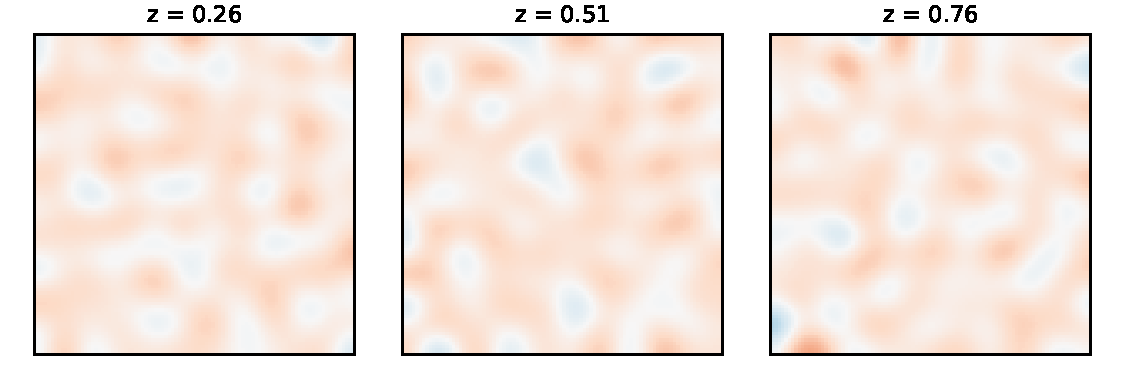
\includegraphics[width=0.62\textwidth]{../figures/cahn_hilliard_3d.pdf}
\caption{Three-dimensional Cahn--Hilliard on $96^3$: slices of the concentration at the final time.}
\end{figure}

\ifincludeproof
\begin{thebibliography}{9}
\bibitem{gantmacher2002oscillation} F.R. Gantmacher, M.G. Krein, Oscillation Matrices and Kernels and Small Vibrations of Mechanical Systems, revised ed., AMS Chelsea Publishing, Providence, RI, 2002.
\bibitem{fallat2011totally} S.M. Fallat, C.R. Johnson, Totally Nonnegative Matrices, Princeton University Press, Princeton, NJ, 2011.
\end{thebibliography}
\fi
\end{document}
